% ------------------------------------------------------------------
\renewcommand{\thisunit}{MATH327 Unit 8}
\renewcommand{\moddate}{Last modified 17 Jan.~2022}
\setcounter{section}{8}
\setcounter{subsection}{0}
\phantomsection
\addcontentsline{toc}{section}{Unit 8: Quantum gases}
\section*{Unit 8: Quantum gases}
\subsection{The photon gas}
Last week we derived the grand-canonical partition function (\eq{eq:partfunc_BE}) that defines quantum Bose--Einstein statistics for systems of non-interacting bosons,
\begin{equation*}
  \ZBE(\be, \mu) = \prod_{\ell = 0}^L \frac{1}{1 - e^{-\be (E_{\ell} - \mu)}}.
\end{equation*}
This expression results from summing over the possible occupation numbers $n_{\ell} \in \Nbb_0$ for each energy level $\cE_{\ell}$ with energy $E_{\ell}$.
The corresponding grand-canonical potential is
\begin{equation*}
  \Phi_{\text{BE}} = -T \log Z_g = T \sum_{\ell = 0}^L \log\left[1 - e^{-\be (E_{\ell} - \mu)}\right],
\end{equation*}
from which we can determine the large-scale properties of the system, including its average internal energy $\vev{E}$, average particle number $\vev{N}$, entropy $S$, and pressure $P$.

To do so, we have to specify the energy levels of the particles that compose the system of interest, and the degeneracies of those energy levels.
One example of this that we have already seen is the analysis of non-relativistic ideal gas particles in \secref{sec:regulate}.
For a single particle with mass $m$ in a volume $V = L^3$, we determined the quantized energies
\begin{equation}
  \label{eq:nonrel_energy}
  E(k_x, k_y, k_z) = \frac{\hbar^2 \pi^2}{2mL^2}\left(k_x^2 + k_y^2 + k_z^2\right),
\end{equation}
where the integers $k_{x, y, z}$ specify the possible momenta of the particle,
\begin{align*}
  \vec p & = (p_x, p_y, p_z) = \hbar \frac{\pi}{L} (k_x, k_y, k_z) &
  k_{x, y, z} & = 1, 2, \cdots.
\end{align*}
(For technical reasons, quantum mechanics requires $k_{x, y, z} \geq 1$, leading us to adjust our ansatz compared to \eq{eq:quant_mom}.)
This system has a unique ground state $\cE_0$ with $\vec k = (1, 1, 1)$ and energy $E_0 = \frac{3}{2} \frac{\hbar^2 \pi^2}{mL^2}$.
The next three energy levels are degenerate, with energy $3 \frac{\hbar^2 \pi^2}{mL^2}$ corresponding to $\vec k = (2, 1, 1)$ and permutations, followed by another three degenerate energy levels with energy $\frac{9}{2} \frac{\hbar^2 \pi^2}{mL^2}$ corresponding to $\vec k = (2, 2, 1)$ and permutations.

This week we will build on that experience to consider a gas of \textit{photons}, massless bosonic quantum particles of light.
For our purposes, with no prior knowledge of particle physics, we can define photons simply by specifying two relevant details of their energy levels.
First, a photon's energy is proportional to the magnitude of its momentum, %with $m = 0$ for massless photons, \eq{eq:nonrel_energy} is clearly problematic.
\begin{equation*}
  \Eph(p) = c \sqrt{p_x^2 + p_y^2 + p_z^2} \equiv c p.
\end{equation*}
Here the speed of light $c$ is really just a unit conversion factor that we could set to $c = 1$ by using appropriate units.
Second, for each momentum $\vec p$, a photon has two degenerate energy levels with the same energy $E(p)$. % TODO: Could mention polarization...

In a volume $V = L^3$, only the same discrete momenta as above are allowed,
\begin{align*}
  p & = \hbar \frac{\pi}{L} \sqrt{k_x^2 + k_y^2 + k_z^2} \equiv \hbar \frac{\pi}{L} k &
  k_{x, y, z} = 1, 2, \cdots,
\end{align*}
so that the quantized photon energies are
\begin{equation}
  \label{eq:photon_Ek}
  \Eph(k) = \hbar c \frac{\pi}{L} k.
\end{equation}
It is conventional to use the speed of light to work with photons in terms of their wavelength \la and angular frequency $\om = 2\pi f$ (not to be confused with generic micro-states $\om_i$), given the relation
\begin{equation*}
  c = \frac{\la \om}{2\pi}.
\end{equation*}
Just like the momenta, the wavelengths \la are also quantized in volume $V = L^3$,
\begin{equation*}
  \la = \frac{2L}{k} \qquad \Lra \qquad c = \frac{\om}{\frac{\pi}{L} k},
\end{equation*}
and we can rewrite \eq{eq:photon_Ek} as
\begin{equation}
  \label{eq:photon_omega}
  \Eph(\om) = \hbar \om.
\end{equation}
Low (\textit{infrared}) frequencies correspond to small energies and long wavelengths, while high (\textit{ultraviolet}) frequencies correspond to large energies and short wavelengths.

We are now ready to write down the grand-canonical potential for a photon gas:
\begin{equation*}
  \Phi_{\text{ph}} = T \sum_{\ell = 0}^L \log\left[1 - e^{-\be (E_{\ell} - \mu)}\right] = 2T \sum_{\vec k} \log\left[1 - e^{-\be (\Eph(k) - \mu)}\right],
\end{equation*}
where the factor of $2$ in the final expression accounts for the doubly degenerate energy levels.
We can simplify this expression by appreciating that photons are easy to create and destroy.
Every time a light is switched on, it begins emitting a constant flood of photons (with wavelengths of several hundred nanometres).
Food in a microwave oven gets hot by absorbing many lower-energy photons (with longer wavelengths around $12$~centimetres).
In both cases an enormous number of photons is required to make even a small change in energy, so that \eq{eq:mu_E} implies the chemical potential of a photon gas must be negligible,
\begin{equation*}
  \mu = \left.\pderiv{E}{N}\right|_S \approx 0 \qquad \Lra \qquad \Phi_{\text{ph}} \approx 2T \sum_{\vec k} \log\left[1 - e^{-\be \Eph(k)}\right].
\end{equation*}
% TODO: This is a significant simplification, and the reason we only consider photons this week...

Another simplification comes from considering the photon gas in a large volume, so that we can approximate the sum over discrete integer $k_{x, y, z}$ by integrals over continuous real $\khat_{x, y, z}$,
\begin{equation*}
  \Phi_{\text{ph}} \approx 2T \int d\khat_x d\khat_y d\khat_z \log\left[1 - e^{-\be \Eph(\khat)}\right].
\end{equation*}
Since the energy $\Eph(\khat)$ depends only on the magnitude $\khat$, we can profit from converting to spherical coordinates.
When we do so, we have to keep in mind that $k_{x, y, z} > 0$ corresponds only to the positive octant of the sphere,
\begin{equation*}
  \int_0^{\infty} d\khat_x \int_0^{\infty} d\khat_y \int_0^{\infty} d\khat_z = \int_0^{\infty} d\khat \; \khat^2 \int_0^{\pi / 2} d\theta \; \sin\theta \int_0^{\pi / 2} d\phi = \frac{\pi}{2} \int_0^{\infty} d\khat \; \khat^2,
\end{equation*}
so that
\begin{equation*}
  \Phi_{\text{ph}} \approx \pi T \int_0^{\infty} d\khat \; \khat^2 \log\left[1 - e^{-\be \Eph(\khat)}\right].
\end{equation*}
We can finally change variables to integrate over the photon angular frequency $\om = c \frac{\pi}{L} k$, with $\Eph = \hbar \om$, to find
\begin{align}
  \Phi_{\text{ph}} & \approx \pi T \left(\frac{L}{\pi c}\right)^3 \int_0^{\infty} d\om \; \om^2 \log\left[1 - e^{-\be \hbar \om}\right] \cr
                   & = \frac{VT}{c^3 \pi^2} \int_0^{\infty} d\om \; \om^2 \log\left[1 - e^{-\be \hbar \om}\right], \label{eq:photon_grand}
\end{align}
recognizing $L^3 = V$.
With this grand-canonical potential derived, we just need to take the appropriate derivatives to determine the thermodynamics and equation of state for the photon gas.
% ------------------------------------------------------------------



% ------------------------------------------------------------------
\subsection{The sun and the void}
We are now ready to analyze the average internal energy from the grand-canonical potential for a photon gas, \eq{eq:photon_grand}.
With $\mu = 0$, \eq{eq:E_grand} from week~6 becomes
\begin{equation*}
  \vev{E}_{\text{ph}} = -T^2 \pderiv{}{T} \left[\frac{\Phi_{\text{ph}}}{T}\right] = \pderiv{}{\be} \left[\be \Phi_{\text{ph}}\right].
\end{equation*}
To begin, we will consider the energy density expressed as an integral over photon frequencies,
\begin{equation*}
  \frac{\vev{E}_{\text{ph}}}{V} = \int_0^{\infty} P(\om) \; d\om,
\end{equation*}
where the function $P(\om)$ is known as the \textit{spectral density}, or simply the \textit{spectrum}.
What is the spectrum for a photon gas?
\begin{mdframed}
  $\displaystyle \frac{\vev{E}_{\text{ph}}}{V} = \frac{1}{c^3 \pi^2} \int_0^{\infty} d\om \; \om^2 \pderiv{}{\be} \log\left[1 - e^{-\be \hbar \om}\right] = $ \\[100 pt]
\end{mdframed}

You should find
\begin{equation}
  \label{eq:Planck_omega}
  P(\om) = \left(\frac{\hbar}{c^3 \pi^2}\right) \frac{\om^3}{e^{\be \hbar \om} - 1},
\end{equation}
which is known as the Planck spectrum, named after Max Planck.
The Planck spectrum is plotted in the figure below, which comes from \href{https://commons.wikimedia.org/wiki/File:Black_body.svg}{Wikimedia Commons}.

\begin{center}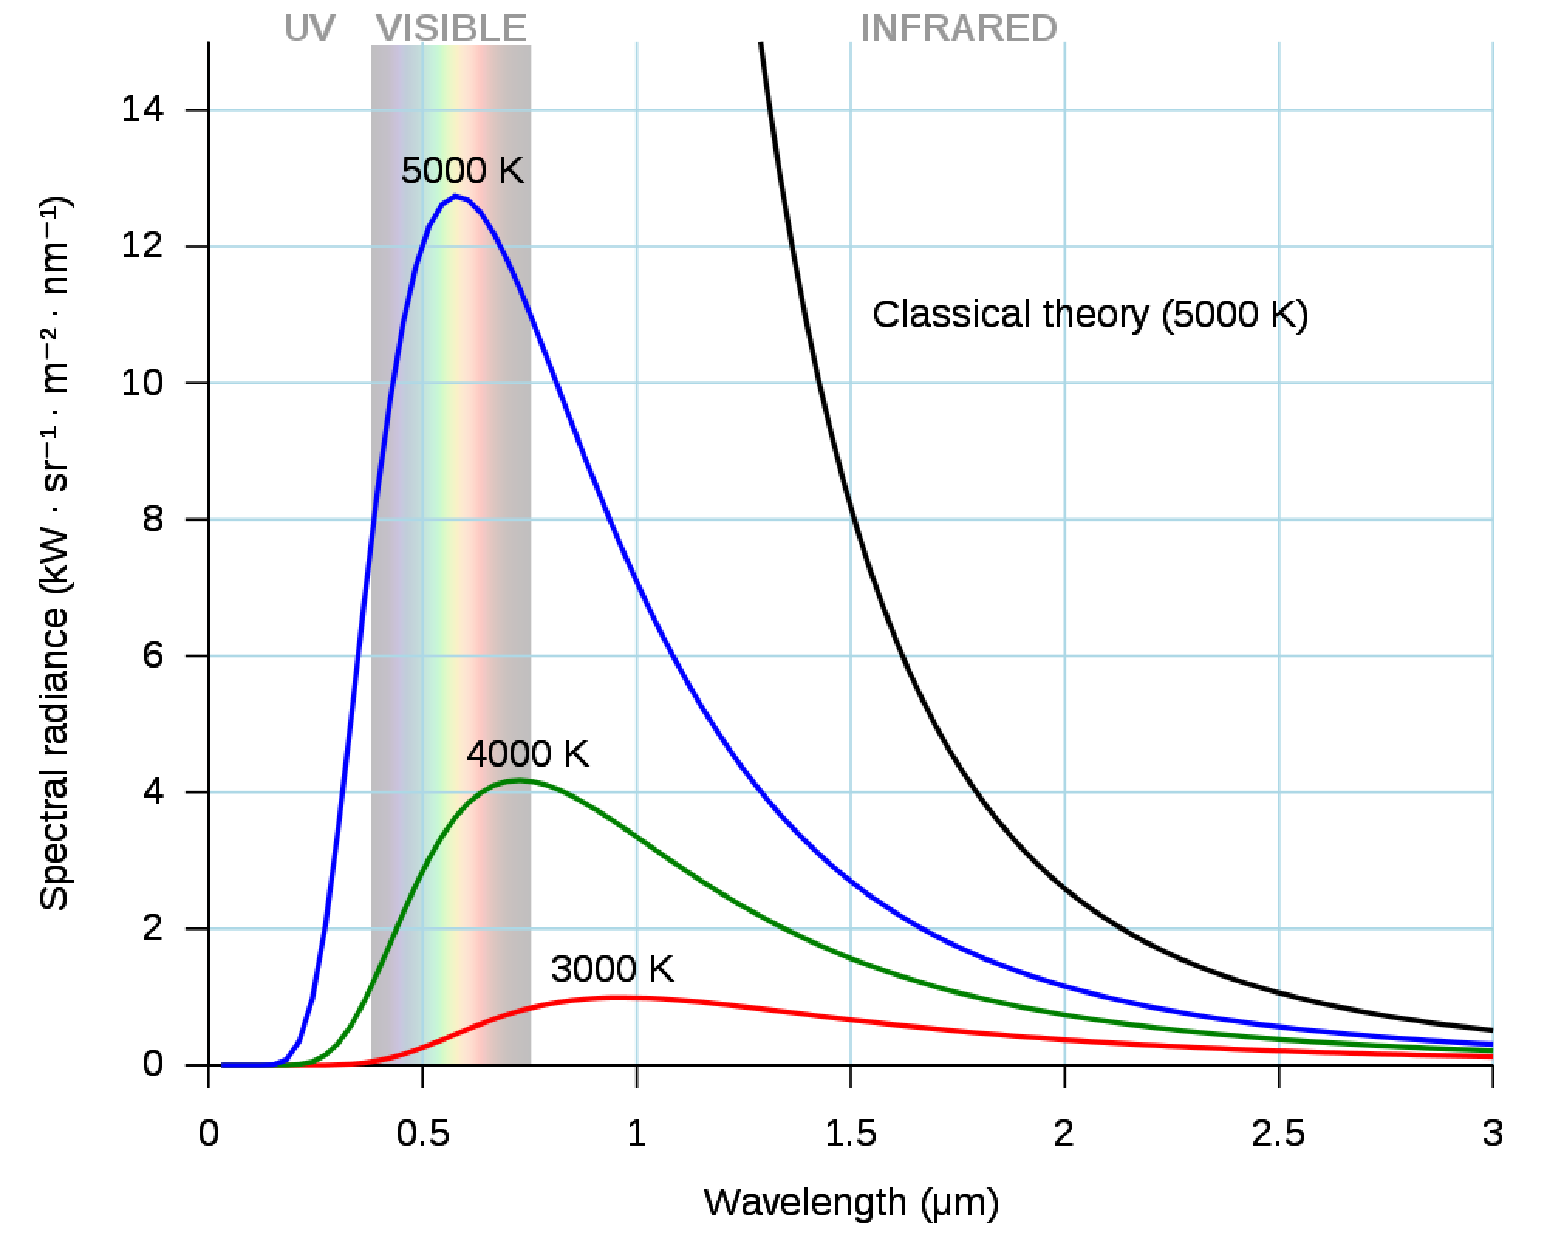
\includegraphics[width=\textwidth]{figs/unit08_spectrum.pdf}\end{center}

In this plot the horizontal axis uses the wavelength $\la = 2\pi c / \om$.
Changing variables in your work above, what is Planck spectrum $P(\la)$ as a function of wavelength?
\begin{mdframed}
  $\displaystyle \frac{\vev{E}_{\text{ph}}}{V} = \frac{\hbar}{c^3 \pi^2} \int_0^{\infty} \frac{\om^3}{e^{\be \hbar \om} - 1} \; d\om = $ \\[120 pt] % WARNING: FORMATTING BY HAND
\end{mdframed}

You should find
\begin{equation}
  \label{eq:Planck_la}
  P(\la) = \left(\frac{16\pi^2 \hbar c}{\la^5}\right) \frac{1}{e^{2\pi\be \hbar c / \la} - 1},
\end{equation}
which is plotted\footnote{The plot divides our $P(\la)$ by $4\pi$~steradian and multiplies it by $c$ to convert from an energy density to a spectral power per unit area per unit of solid angle.  For our purposes only the functional form is significant.} for three temperatures $T = 1 / \be$ in the figure above.
Considering first the high-energy ultraviolet (UV) limit of small wavelengths $\la$, we can see from \eq{eq:Planck_la} that $P(\la)$ is exponentially suppressed, which overwhelms the diverging factor $\propto 1 / \la^5$ in parentheses.

In the low-energy infrared limit, the large $\la$ has the same effect that a large temperature ($\be \ll 1$) would have: $e^{2\pi\be \hbar c / \la} - 1 \approx 2\pi\be \hbar c / \la$ and
\begin{equation*}
  P(\la) \approx \left(\frac{16\pi^2 \hbar c}{\la^5}\right) \frac{\la}{2\pi\be \hbar c} = \frac{8\pi T}{\la^4}.
\end{equation*}
The connection to large temperatures indicates that this is what classical statistics would predict for the energy spectrum of light.
It is known as the Rayleigh--Jeans spectrum, named after \href{https://en.wikipedia.org/wiki/John_William_Strutt,_3rd_Baron_Rayleigh}{the third Baron Rayleigh} and \href{https://en.wikipedia.org/wiki/James_Jeans}{James Jeans}.
Recall that the classical approach sums over all possible energies for each degree of freedom, corresponding to a light-emitting object (historically known as a \textit{black body}) emitting light of all wavelengths $\la$.
According to the classical Rayleigh--Jeans spectrum, in the limit $\la \to 0$ this light would carry an infinite amount of energy, an obvious error that became known as the \textit{ultraviolet catastrophe}.
Planck's (heuristic) solution to this conundrum in 1900 was one of the first steps towards the quantum physics that introduces the exponential suppression we computed above.

One final observation we will make about the Planck spectrum shown above is that as the temperature increases, the maximum of the Planck spectrum moves to shorter wavelengths and correspondingly larger energies.
The fact that the peak of the spectrum for $T \approx 5000$~K falls within the wavelengths of visible light (roughly $400$--$700$~nm) is not a coincidence.
As shown in the figure below (from \href{https://commons.wikimedia.org/wiki/File:Solar_Spectrum.png}{Wikimedia Commons}), the amount of sunlight that reaches the surface of the earth is also maximized around visible wavelengths, which are visible to us because we have evolved to make the most efficient use of this sunlight.

Taking into account the absorption of some sunlight by molecules in the atmosphere, we can see from the figure below that the energy spectrum of the sunlight reaching the top of the atmosphere is quite close to a Planck (or `blackbody') spectrum with temperature $T \approx 5778$~K.
The agreement isn't perfect, which is to be expected since the Planck spectrum relies on the non-trivial assumption of an ideal gas of non-interacting particles.
Even with that caveat, numerically fitting the measured sunlight to the Planck spectrum is how the surface temperature of the sun is determined to be $T \approx 5778$~K.
This same fitting procedure can even be done for distant stars, with red stars corresponding to relatively low temperatures $T \lesssim 3500$~K and blue stars corresponding to relatively high temperatures $T \gtrsim 10{,}000$~K.

\begin{center}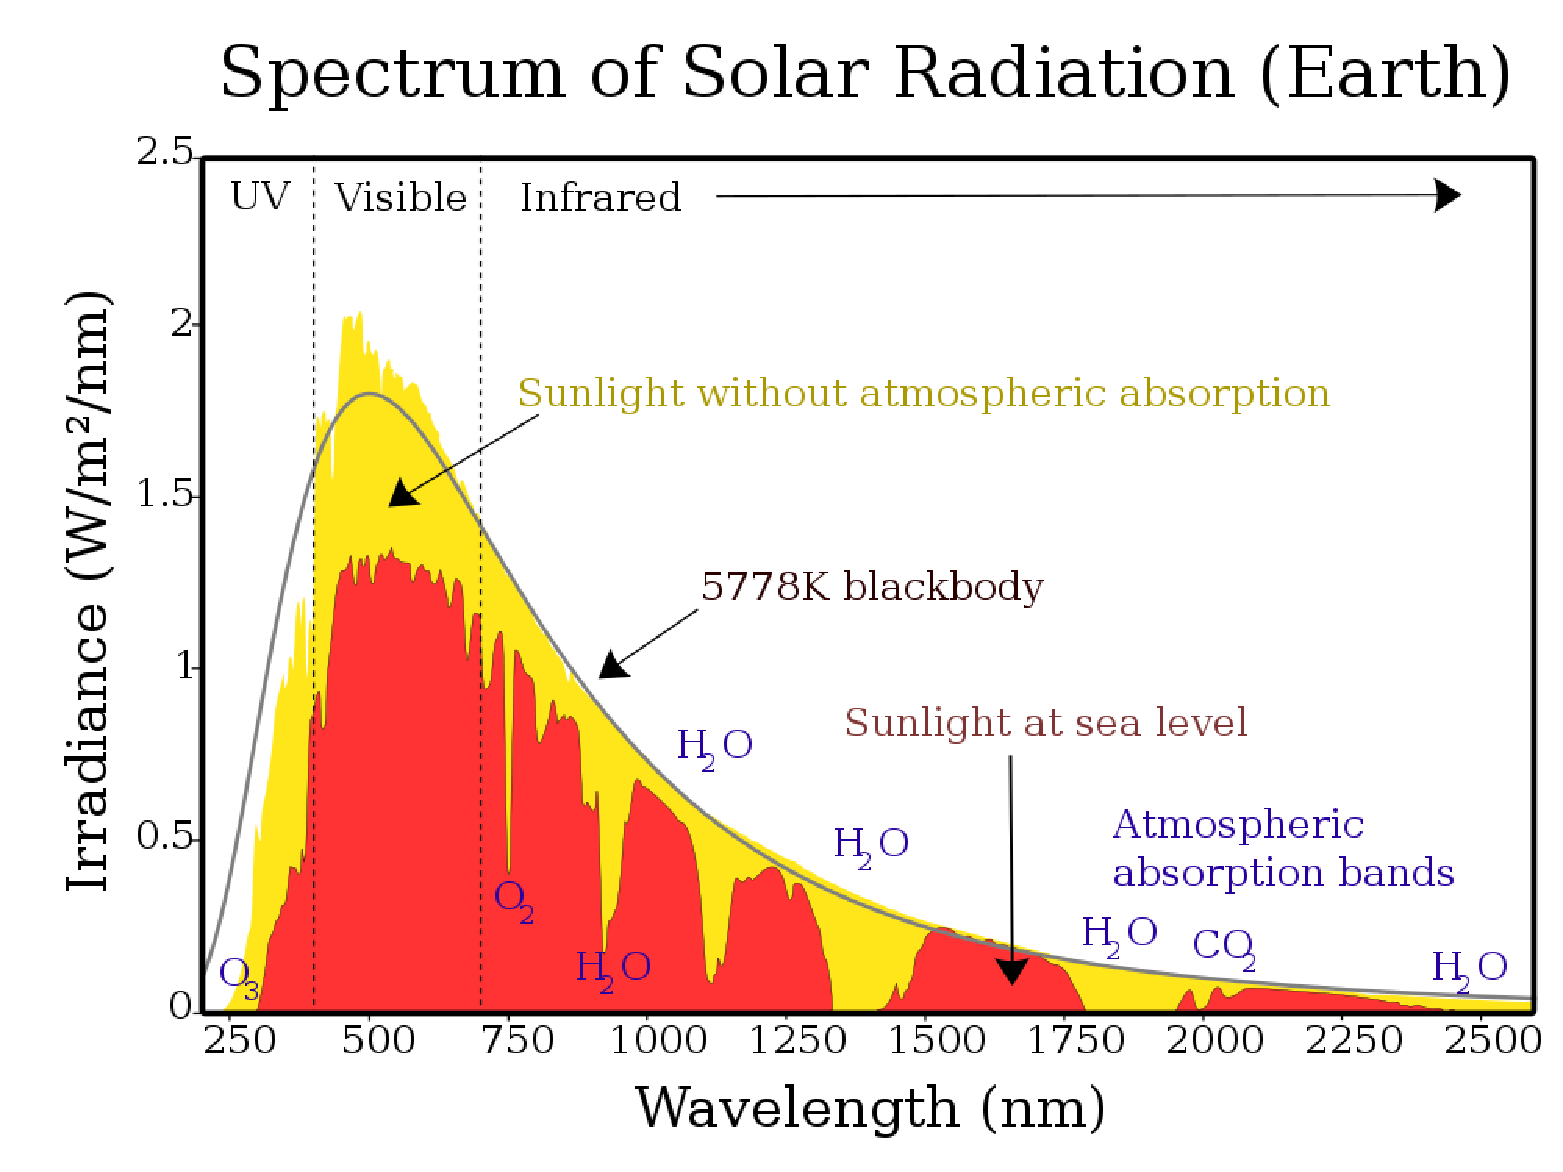
\includegraphics[width=\textwidth]{figs/unit08_sun.pdf}\end{center}

In fact, we can even use the Planck spectrum to determine the temperature of inter-galactic space.
Rather than being empty, these voids are actually permeated by a very low-temperature photon gas left over from the Big Bang roughly $14$~billion years ago.
This photon gas is known as the \href{https://en.wikipedia.org/wiki/Cosmic_microwave_background}{cosmic microwave background} (CMB), and carries information about the early evolution of the universe, including some of the strongest evidence for the existence of dark matter.

The picture below is a famous visualization of the CMB, provided by the \href{http://www.esa.int/ESA_Multimedia/Images/2013/03/Planck_CMB}{European Space Agency} and produced from measurements taken by their `Planck' satellite. % Can compare with WMAP from wmap.gsfc.nasa.gov/media/101080/
To produce this image, for each point in the sky the satellite measures the photon spectrum reaching it from that direction.
The contributions coming from stars and galaxies are subtracted, and the remaining data is fit to the Planck spectrum to find the temperature of the intergalactic CMB photon gas at that point.
From point to point, there are only small temperature fluctuations around the average $T_{\text{CMB}} \approx 2.725$~K.
That average temperature is subtracted and the fluctuations themselves are shown below, with warmer red-coloured regions only $\De T \approx 0.0002$~K hotter than the cooler blue-coloured regions.

\begin{center}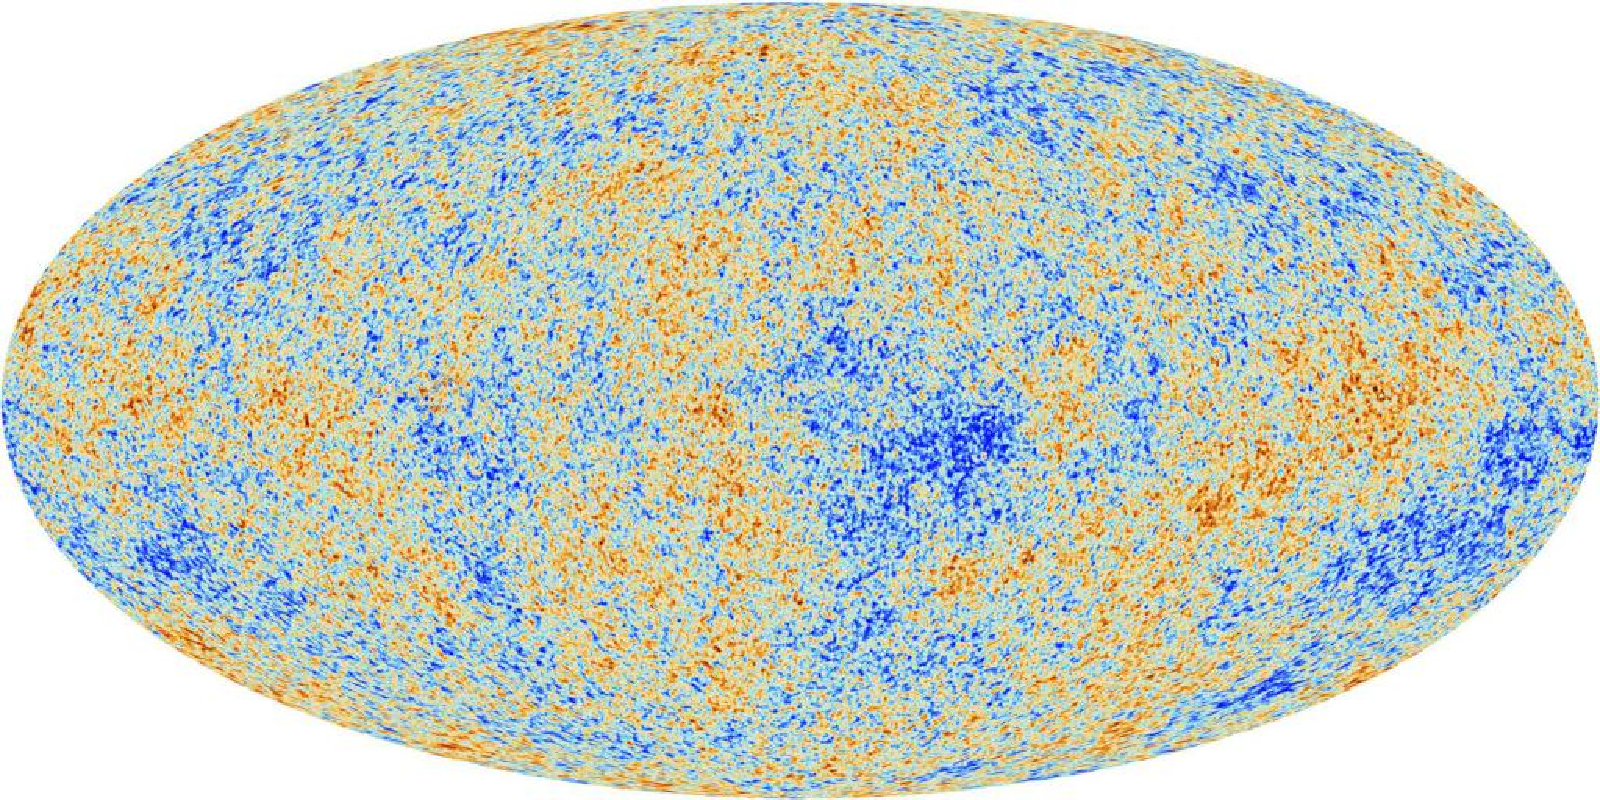
\includegraphics[width=\textwidth]{figs/unit08_CMB.pdf}\end{center}

The final figure below illustrates such a fit of CMB data to the Planck spectrum, using measurements taken by the Cosmic Background Explorer (COBE) satellite and \href{https://doi.org/10.1086/185717}{published in 1990}.
(This version of the figure is adapted from that publication, and copied from Schroeder's \textit{Introduction to Thermal Physics}.)
The squares are the measured data, and their size represents a cautious estimate of uncertainties.
They are plotted with the frequency $f = \om / (2\pi)$ on the horizontal axis, with $f \approx 3\cdot 10^{-11}~\text{s}^{-1}$ corresponding to a low-energy wavelength $\la = c / f \approx 1$~mm, roughly $1000$ times longer than the wavelengths of visible light.
The solid line is a fit to the data that produces $T_{\text{CMB}} = 2.735 \pm 0.060$~K.
While more recent satellites have increased the precision with which we know $T_{\text{CMB}}$, this first result was awarded the 2006 Nobel Prize in Physics.

\begin{center}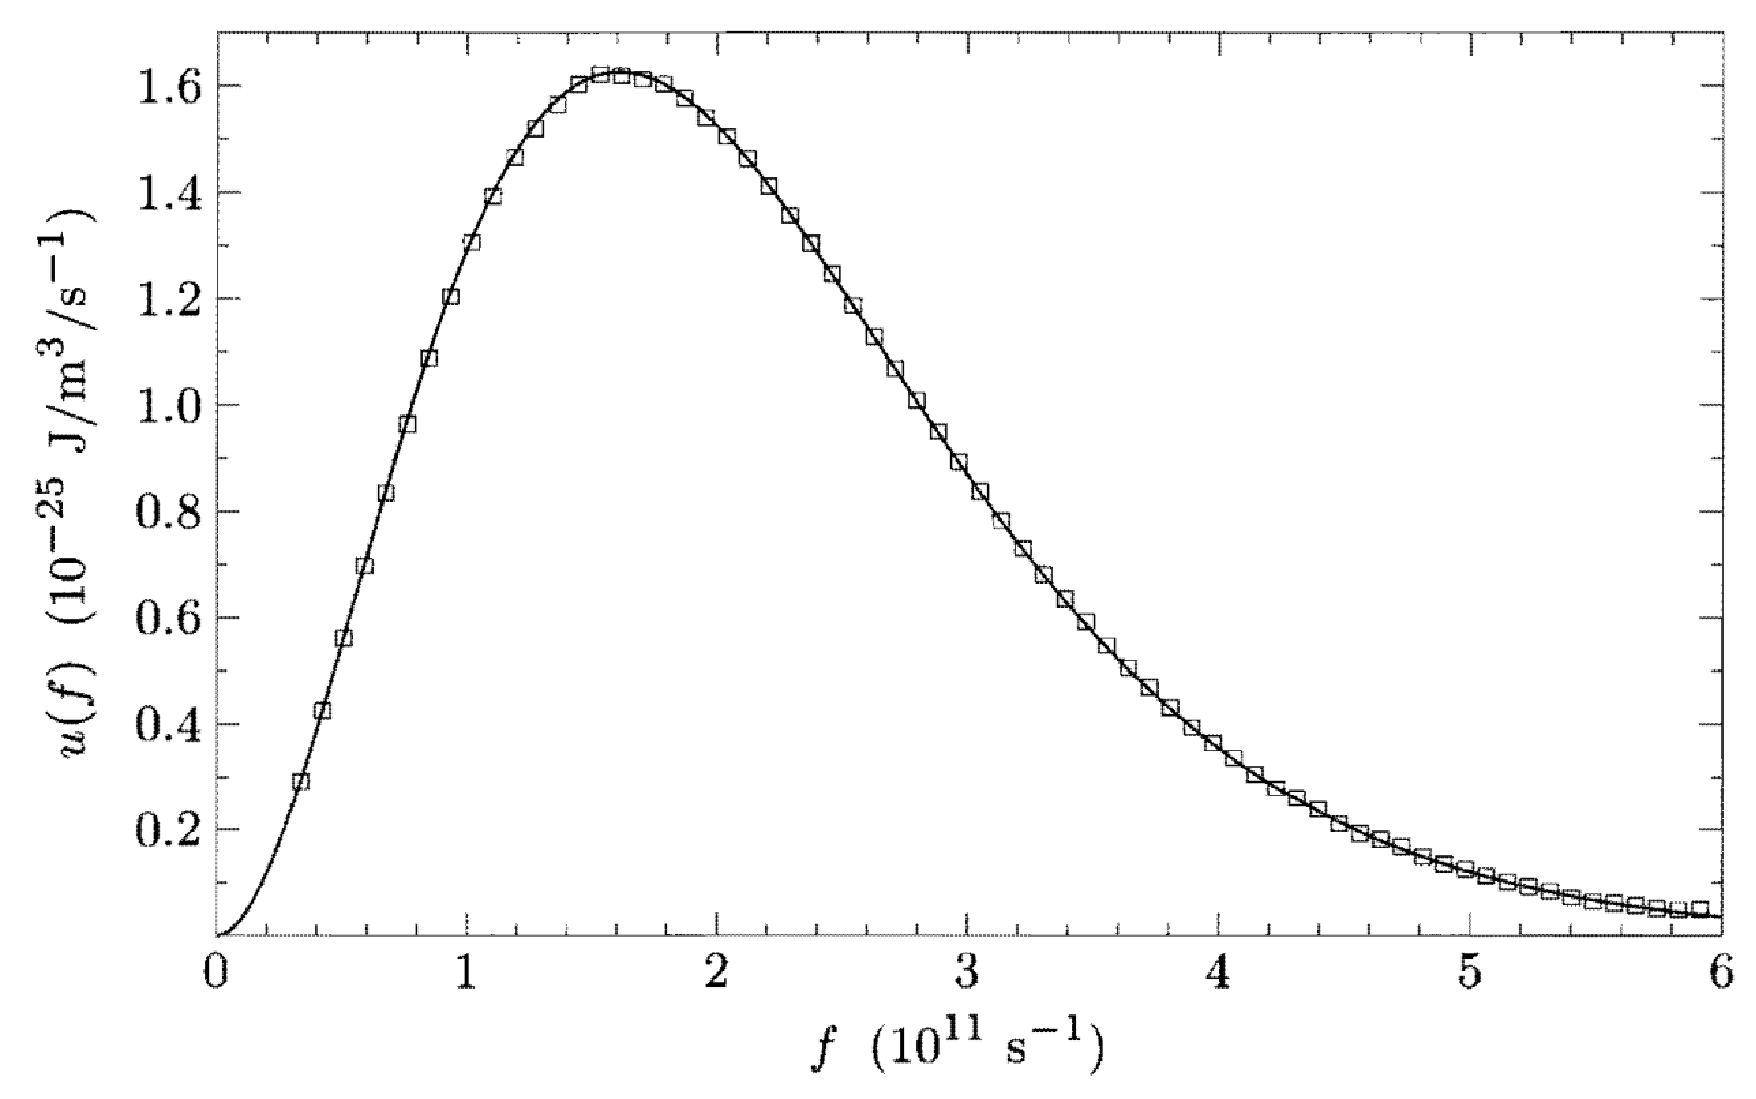
\includegraphics[width=\textwidth]{figs/unit08_COBE.pdf}\end{center}

\begin{shaded}
  Even though we derived the Planck spectrum by assuming an ideal gas of non-interacting photons, we see that it provides an excellent mathematical model for real physical systems, stretching from the hottest to the coldest places in the universe.
\end{shaded}
% ------------------------------------------------------------------



% ------------------------------------------------------------------
\subsection{Equation of state for the photon gas}
Having looked in some detail at the integrand for the photon gas energy density, \eq{eq:Planck_omega}, let's complete the integration, which involves a famous integral related to the Riemann zeta function:
\begin{equation*}
  I_4 = \int_0^{\infty} \frac{x^3}{e^x - 1} dx = \Gamma(4) \zeta(4) = \frac{\pi^4}{15}.
\end{equation*}
Using this result, what is the ideal photon gas energy density?
\begin{mdframed}
  $\displaystyle \frac{\vev{E}_{\text{ph}}}{V} = \frac{\hbar}{c^3 \pi^2} \int_0^{\infty} \frac{\om^3}{e^{\be \hbar \om} - 1} \; d\om = $ \\[100 pt]
\end{mdframed}

You should find a result proportional to $T^4$.
It would be ideal (sorry) if we could put this in a form as simple as \eq{eq:ideal_energy} for the energy of an $N$-particle non-relativistic ideal gas in the canonical ensemble.
Now that we are working in the grand-canonical ensemble, this requires computing the average photon number from \eq{eq:N_grand},
\begin{equation*}
  \vev{N}_{\text{ph}} = -\left. \pderiv{}{\mu} \Phi_{\text{ph}}\right|_{\mu = 0} = -\left. \frac{VT}{c^3 \pi^2} \int_0^{\infty} d\om \; \om^2 \pderiv{}{\mu} \log\left[1 - e^{-\be \hbar \om} e^{\be \mu}\right] \right|_{\mu = 0}.
\end{equation*}
recalling $\mu = 0$ for photon gases.
The calculation is quite similar to that for the average internal energy density, now involving the integral
\begin{equation*}
  I_3 = \int_0^{\infty} \frac{x^2}{e^x - 1} dx = \Gamma(3) \zeta(3) = 2\zeta(3).
\end{equation*}
\newpage % WARNING: FORMATTING BY HAND
\noindent Using this result, what is the ideal photon gas number density?
\begin{mdframed}
  $\displaystyle \frac{\vev{N}_{\text{ph}}}{V} = \frac{1}{c^3 \pi^2} \int_0^{\infty} \frac{\om^2}{e^{\be \hbar \om} - 1} \; d\om = $ \\[100 pt]
\end{mdframed}

You should find a result proportional to $T^3 \propto \vev{E}_{\text{ph}} / T$, so that
\begin{equation}
  \vev{E}_{\text{ph}} = \frac{\pi^2}{15 \hbar^3 c^3} VT^4 = \frac{\pi^4}{30\zeta(3)} \vev{N}_{\text{ph}} T.
\end{equation}
The functional form is the same as \eq{eq:ideal_energy}, with a larger numerical factor
\begin{equation*}
  \frac{\pi^4}{30\zeta(3)} = \frac{\Gamma(4) \zeta(4)}{\Gamma(3) \zeta(3)} \approx 2.7
\end{equation*}
compared to the $\frac{3}{2}$ for the classical non-relativistic case.

To get the rest of the way to the equation of state for the photon gas, we need to compute the \textit{radiation pressure}
\begin{equation*}
  P_{\text{ph}} = -\left. \pderiv{}{V} \vev{E}_{\text{ph}} \right|_{S_{\text{ph}}},
\end{equation*}
which requires first figuring out the condition of constant entropy $S_{\text{ph}}$ for a photon gas.
From \eq{eq:grand_relation} with $\mu = 0$, we have
\begin{equation*}
  S_{\text{ph}} = \frac{\vev{E}_{\text{ph}} - \Phi_{\text{ph}}}{T}.
\end{equation*}
Looking back to \eq{eq:photon_grand} for the grand-canonical potential, we see
\begin{equation*}
  \frac{\Phi_{\text{ph}}}{T} = \frac{V}{c^3 \pi^2} \int_0^{\infty} d\om \; \om^2 \log\left[1 - e^{-\be \hbar \om}\right] = \frac{VT^3}{\hbar^3 c^3 \pi^2} \int_0^{\infty} dx \; x^2 \log\left[1 - e^{-x}\right],
\end{equation*}
changing variables to $x = \be \hbar \om = \hbar \om / T$.
The final factor in this expression is yet another delightful integral,
\begin{equation*}
  \int_0^{\infty} dx \; x^2 \log\left[1 - e^{-x}\right] = -2\zeta(4) = -\frac{\pi^4}{45}.
\end{equation*}
Since this gives us $S \propto VT^3$, we can conclude that the condition of constant entropy for a photon gas is $V T^3 = \mbox{constant}$, in contrast to the $V T^{3/2}$ dependence of \eq{eq:ideal_entropy} for classical non-relativistic particles.

\newpage % WARNING: FORMATTING BY HAND
At this point we just need to insert the constant-entropy condition $T = b V^{-1 / 3}$ (with $b$ a constant) into the average internal energy and take the derivative:
\begin{mdframed}
  $\displaystyle P = -\left. \pderiv{}{V} \vev{E}_{\text{ph}} \right|_{S_{\text{ph}}} = -\pderiv{}{V} \frac{\pi^2}{15 \hbar^3 c^3} b^4 V^{-1 / 3} = $ \\[100 pt]
\end{mdframed}
You should find the following equation of state for the photon gas,
\begin{equation}
  P_{\text{ph}} V = \frac{1}{3} \vev{E}_{\text{ph}} = \frac{\pi^4}{90\zeta(3)} \vev{N}_{\text{ph}} T.
\end{equation}
The functional form is the same as the (classical, non-relativistic) ideal gas law, with just an additional numerical factor
\begin{equation*}
  \frac{\pi^4}{90\zeta(3)} = \frac{\zeta(4)}{\zeta(3)}.
\end{equation*}
% ------------------------------------------------------------------



% ------------------------------------------------------------------
\subsection{\label{sec:fermi_nonrel}Non-relativistic ideal fermion gas}
This week we wrap up our applications of the grand-canonical ensemble to investigate ideal gases of non-interacting particles.
We again take the quantum statistical approach of defining micro-states by summing over the possible occupation numbers $n_{\ell}$ for each energy level $\cE_{\ell}$ with energy $E_{\ell}$.
In contrast to the bosonic case considered last week, we now focus on quantum gases of fermions, where the only possible occupation numbers are $n_{\ell} = 0$ and $1$, since the Pauli exclusion principle prevents multiple identical fermions from occupying the same energy level.

In \secref{sec:fermi} we derived the grand-canonical partition function (\eq{eq:partfunc_FD}) that defines quantum Fermi--Dirac statistics for such systems of non-interacting fermions,
\begin{equation*}
  \ZFD(\be, \mu) = \prod_{\ell = 0}^L \left[1 + e^{-\be (E_{\ell} - \mu)}\right],
\end{equation*}
for inverse temperature $\be = 1 / T$ and chemical potential $\mu$.
Recall that it is possible for systems of fermions to have any value for the chemical potential (either positive or negative), in contrast to the systems of bosons we considered last week.
From the corresponding grand-canonical potential,
\begin{equation*}
  \Phi_{\text{FD}} = -T \sum_{\ell = 0}^L \log\left[1 + e^{-\be (E_{\ell} - \mu)}\right]
\end{equation*}
we can determine the large-scale properties of the system, including its average internal energy $\vev{E}$, average particle number $\vev{N}$, entropy $S$, and pressure $P$, along with the equation of state relating these quantities.

A concrete calculation requires specifying the energy levels of the particles that compose the gas, and the degeneracies of those energy levels.
Let's begin this week by considering non-relativistic particles of the sort we previously analyzed in \secref{sec:regulate}.
In a volume $V = L^3$, the energy levels are defined by the non-zero quantized energies
\begin{align*}
  E(k) & = \frac{p^2}{2m} = \frac{\hbar^2 \pi^2}{2mL^2}\left(k_x^2 + k_y^2 + k_z^2\right) &
  k_{x, y, z} & = 1, 2, \cdots.
\end{align*}
In addition to the usual degeneracies coming from permutations of $(k_x, k_y, k_z)$ that we discussed in previous weeks, for each distinct $\vec k$ typical fermions such as electrons have two degenerate energy levels with the same energy.
This factor of $2$ has a different origin compared to the double degeneracy discussed for photons last week.
Rather than worry about the physical origins of this behaviour, in both cases we simply incorporate this given information into our ansatz. % TODO: Could mention spin...

The grand-canonical potential for an ideal gas of non-relativistic fermions is therefore
\begin{equation*}
  \Phi_{\text{f}} = T \sum_{\ell = 0}^L \log\left[1 + e^{-\be (E_{\ell} - \mu)}\right] = 2T \sum_{\vec k} \log\left[1 + \exp\left(-\frac{\hbar^2 \pi^2 k^2}{2mL^2 T} + \frac{\mu}{T}\right)\right].
\end{equation*}
We can again proceed by considering the gas in a large volume and approximating the sum over discrete integer $k_{x, y, z}$ by integrals over continuous real $\khat_{x, y, z}$:
\begin{equation*}
  \Phi_{\text{f}} \approx 2T \int d\khat_x d\khat_y d\khat_z \log\left[1 + \exp\left(-\frac{\hbar^2 \pi^2 \khat^2}{2mL^2 T} + \frac{\mu}{T}\right)\right].
\end{equation*}
Converting to spherical coordinates and carrying out the angular integrations over the $\frac{\pi}{2}$ solid angle of the octant of the sphere with $k_{x, y, z} > 0$, we have
\begin{equation*}
  \Phi_{\text{f}} \approx \pi T \int_0^{\infty} d\khat \; \khat^2 \log\left[1 + \exp\left(-\frac{\hbar^2 \pi^2 \khat^2}{2mL^2 T} + \frac{\mu}{T}\right)\right].
\end{equation*}
In the same spirit as the change of variables we carried out last week, to integrate over photon frequencies $\om = \Eph / \hbar$, we will now change variables to integrate over the fermion energy:
\begin{align*}
  E = \frac{\hbar^2 \pi^2}{2mL^2}\khat^2 \quad \lra \quad \khat & = \frac{L\sqrt{m}}{\pi \hbar} \sqrt{2E} \cr
                                                         d\khat & = \frac{L\sqrt{m}}{\pi \hbar} \frac{dE}{\sqrt{2E}}.
\end{align*}
Plugging this in produces
\begin{align}
  \Phi_{\text{f}} & \approx \pi T \left(\frac{L^3 m^{3 / 2}}{\pi^3 \hbar^3}\right) \int_0^{\infty} dE \frac{2E}{\sqrt{2E}} \log\left[1 + e^{-\be(E - \mu)}\right] \cr
                  & = \frac{\sqrt{2 m^3} VT}{\pi^2 \hbar^3} \int_0^{\infty} dE \sqrt{E} \log\left[1 + e^{-\be(E - \mu)}\right]. \label{eq:fermi_grand}
\end{align}
recognizing $L^3 = V$.

With this grand-canonical potential derived, we just need to take the appropriate derivatives to determine the thermodynamics and equation of state for non-relativistic fermions.
When doing so, we'll focus on the low-temperature regime where we expect quantum Fermi--Dirac statistics to differ significantly from the classical case we considered back in \secref{sec:regulate}.
As we saw in \secref{sec:quantum_classical}, at high temperatures (with large negative chemical potential) the classical approach provides a good approximation to the true quantum physics.
% TODO: Low temperatures provide a significant simplification, which is why we only consider that regime this week
% ------------------------------------------------------------------



% ------------------------------------------------------------------
\subsection{Low-temperature equation of state}
Rather than the average internal energy $\vev{E}_{\text{f}}$, it will prove profitable to first analyze the average particle number
\begin{equation*}
  \vev{N}_{\text{f}} = -\pderiv{}{\mu} \Phi_{\text{f}}
\end{equation*}
coming from the grand-canonical potential for non-relativistic fermions, \eq{eq:fermi_grand}.
In analogy to the Planck spectrum we derived for the photon gas last week, we first express the particle number density as an integral over energies,
\begin{equation*}
  \frac{\vev{N}_{\text{f}}}{V} = \frac{\sqrt{2m^3}}{\pi^2 \hbar^3} \int_0^{\infty} F(E) \sqrt{E} \; dE,
\end{equation*}
where the function $F(E)$ is known as the Fermi function.
In contrast to the Planck spectrum, all the constant factors are kept separate from $F(E)$:
\begin{align}
  \frac{\vev{N}_{\text{f}}}{V} & = \frac{\sqrt{2m^3} T}{\pi^2 \hbar^3} \int_0^{\infty} dE \sqrt{E} \pderiv{}{\mu} \log\left[1 + e^{-\be(E - \mu)}\right] \cr
                               & = \frac{\sqrt{2m^3}}{\pi^2 \hbar^3} \int_0^{\infty} \frac{1}{e^{\be(E - \mu)} + 1} \sqrt{E} \; dE = \frac{\sqrt{2m^3}}{\pi^2 \hbar^3} \int_0^{\infty} F(E) \sqrt{E} \; dE. \label{eq:N_fermi}
\end{align}
This allows the Fermi function to closely resemble the average occupation numbers $\vev{n_{\ell}}$ we computed in \secref{sec:quantum_classical}:
\begin{equation}
  \label{eq:Fermi_func}
  F(E) = \frac{1}{e^{\be(E - \mu)} + 1}.
\end{equation}

As usual in the grand-canonical approach, the average particle number and Fermi function depend on both the inverse temperature \be and the chemical potential $\mu$.
Expressing $F(E)$ in terms of the dimensionless ratios $E / \mu$ and $T / \mu$,
\begin{equation*}
  F(E) = \frac{1}{\exp\left[\frac{E - \mu}{T}\right] + 1} = \frac{1}{\exp\left[\frac{\mu}{T}\left(\frac{E}{\mu} - 1\right)\right] + 1} = \frac{1}{\left(\exp\left[\frac{E}{\mu} - 1\right]\right)^{\mu / T} + 1},
\end{equation*}
we can highlight the two main features of the figure below, which plots the Fermi function against $E / \mu$ for various temperatures $T / \mu$.

\begin{center}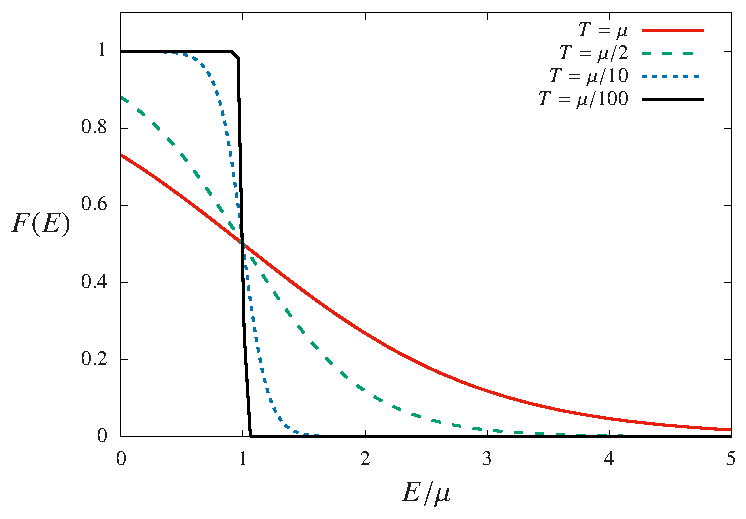
\includegraphics[width=\textwidth]{figs/unit08_dist.pdf}\end{center}

First, we can see that the point $E = \mu$, where $F(E) = 1 / 2$ for any non-zero temperature, is a threshold at which the behaviour of the Fermi function changes.
For larger energies $E > \mu$, the exponential factor $\exp\left[\frac{E}{\mu} - 1\right] > 1$ and drives $F(E) \to 0$ as the energy increases.
For smaller energies $E < \mu$, the exponential factor $\exp\left[\frac{E}{\mu} - 1\right] < 1$ and vanishes as the energy decreases, leaving $F(E) \to 1$.
These two asymptotic limits reflect the possible energy level occupation numbers for fermions, $n_{\ell} = 0$ and $1$.
Second, smaller temperatures cause much more rapid approach to these two limits, with the exponential factor either enhanced (if $E > \mu$) or suppressed (if $E < \mu$) by a power $\mu / T \gg 1$.
Therefore, for small temperatures $T \ll \mu$, we can simplify our calculations by approximating the Fermi function as a step function,
\begin{equation}
  \label{eq:Fermi_step}
  F(E) \approx \left\{\begin{array}{l}1 \qquad \mbox{for } \ E < \mu \\
                                      0 \qquad \mbox{otherwise}\end{array}\right. .
\end{equation}
Using this approximation, what is the resulting particle number density?
\begin{mdframed}
  $\displaystyle \frac{\vev{N}_{\text{f}}}{V} = \frac{\sqrt{2m^3}}{\pi^2 \hbar^3} \int_0^{\infty} F(E) \sqrt{E} \; dE = $ \\[100 pt]
\end{mdframed}

You should find a result proportional to $\mu^{3 / 2}$ but independent of $T$.
The temperature independence can be understood by viewing this as the leading-order term in an expansion in the small temperature (known as a \textit{Sommerfeld expansion}, named after \href{https://en.wikipedia.org/wiki/Arnold_Sommerfeld}{Arnold Sommerfeld}).
The $\mu^{3 / 2}$ dependence on the chemical potential is also what we would predict even without doing the detailed calculation.
The step function in \eq{eq:Fermi_step} corresponds to a single fermion occupying each and every energy level with $E_{\ell} < \mu$, while all energy levels with $E_{\ell} > \mu$ are unoccupied.
Since $E(k) \propto k^2$, summing over all $k_{x, y, z}$ corresponds to computing (a portion of) the volume of a sphere of radius $r = \sqrt{\mu}$, which is proportional to $r^3 = \mu^{3 / 2}$ as we found directly above.
If we were to invert this relation, we would obtain the so-called \textbf{Fermi energy} as a function of the particle number density,
\begin{equation}
  \label{eq:Fermi_energy}
  E_F = \mu = \frac{\hbar^2}{2m}\left(\frac{3\pi^2 \vev{N}_{\text{f}}}{V}\right)^{2 / 3}.
\end{equation}

Now we can consider the average energy density of the non-relativistic fermion gas at low temperatures.
Rather than taking another derivative of the grand-canonical potential, we can note from \eq{eq:total_energy_levels} and from our work on the photon gas last week that
\begin{equation}
  \frac{\vev{E}_{\text{f}}}{V} = \frac{\sqrt{2m^3}}{\pi^2 \hbar^3} \int_0^{\infty} E \; F(E) \sqrt{E} \; dE.
\end{equation}
That is, instead of simply counting the number of fermions in the system, we need to add up their energies, introducing an extra factor of $E$ compared to \eq{eq:N_fermi}.
Still using the low-temperature step-function approximation for the Fermi function in \eq{eq:Fermi_step}, what is the average energy density?
\begin{mdframed}
  $\displaystyle \frac{\vev{E}_{\text{f}}}{V} = \frac{\sqrt{2m^3}}{\pi^2 \hbar^3} \int_0^{\infty} F(E) E^{3 / 2} \; dE = $ \\[100 pt]
\end{mdframed}

You should find
\begin{equation}
  \label{eq:fermi_E_N}
  \vev{E}_{\text{f}} = \frac{3}{5} \mu \vev{N}_{\text{f}},
\end{equation}
which means that the average energy of the fermions in a low-temperature ideal gas is $3 / 5$ the Fermi energy $E_F = \mu$.
In particular, because this result is also independent of the temperature, we find that non-interacting quantum fermions retain a positive energy even as the temperature approaches absolute zero, $T \to 0$.
This can be understood by recalling that the lowest-energy pair of degenerate energy levels can each only hold a single fermion, forcing all additional fermions to `fill' energy levels with larger energies $E_{\ell} > 0$, up to the Fermi energy set by the chemical potential.
This is a stark contrast to the classical ($\vev{E} \propto T$) and bosonic ($\vev{E} \propto T^4$) cases we considered earlier, where the average energy vanishes in the zero-temperature limit.
As discussed in Sections~\ref{sec:spin_info} and \ref{sec:quantum_classical}, in those cases all the particles in the system are able to fall into the lowest energy level, with only an exponentially small probability for particles to occupy any energy levels with $E_{\ell} > E_0$.

To get the rest of the way to the equation of state for the ideal gas of non-relativistic fermions, we need to compute the pressure
\begin{equation*}
  P_{\text{f}} = -\left. \pderiv{}{V} \vev{E}_{\text{f}} \right|_{N, S_{\text{f}}}.
\end{equation*}
In the low-temperature limit, the condition of constant entropy $S_{\text{f}} = -\sum_{i = 1}^M p_i \log p_i$ is automatically satisfied, since the step function in \eq{eq:Fermi_step} restricts the system to a single micro-state, resulting in $S_{\text{f}} = 0$.
This micro-state is the one in which each and every energy level with $E_{\ell} < \mu$ is occupied, while all energy levels with $E_{\ell} > \mu$ are unoccupied.

Inserting \eq{eq:Fermi_energy} into \eq{eq:fermi_E_N}, we have
\begin{equation*}
  \vev{E}_{\text{f}} = \frac{3}{5} \mu \vev{N}_{\text{f}} = \frac{3}{5} \left(\frac{\hbar^2}{2m}\right) \left(\frac{3\pi^2}{V}\right)^{2 / 3} \vev{N}_{\text{f}}^{5 / 3}.
\end{equation*}
The pressure is therefore
\begin{align}
  P_{\text{f}} & = -\pderiv{}{V} \left[\frac{3}{5} \left(\frac{\hbar^2}{2m}\right) \left(\frac{3\pi^2}{V}\right)^{2 / 3} \vev{N}_{\text{f}}^{5 / 3}\right] = \frac{2}{3V} \left[\frac{3}{5} \left(\frac{\hbar^2}{2m}\right) \left(\frac{3\pi^2}{V}\right)^{2 / 3} \vev{N}_{\text{f}}^{5 / 3}\right] \nonumber \\
               & = \left(3\pi^2\right)^{2 / 3} \frac{\hbar^2}{5m} \left(\frac{\vev{N}_{\text{f}}}{V}\right)^{5 / 3} = \frac{2}{5} \mu \frac{\vev{N}_{\text{f}}}{V} = \frac{2}{3} \frac{\vev{E}_{\text{f}}}{V}.
\end{align}
The three expressions in the second line above present several relations between the pressure, the energy density, the Fermi energy $E_F = \mu$ and the particle number density.
In particular, we can see that the pressure (like the energy) remains positive even as the temperature approaches absolute zero, with
\begin{equation}
  \label{eq:degen_pressure}
  P_{\text{f}} = \left(3\pi^2\right)^{2 / 3} \frac{\hbar^2}{5m} \rho_{\text{f}}^{5 / 3},
\end{equation}
where we define the density $\rho_{\text{f}} = \vev{N}_{\text{f}} / V$.
This positive pressure in the zero-temperature limit is not due to any direct force between the fermions, which remain non-interacting in this ideal gas.
Instead, it is a purely quantum effect resulting from the Pauli exclusion principle.

As we saw earlier in this section, the temperature independence of the pressure $P_{\text{f}}$ is due to approximating the low-temperature Fermi function as a step function in \eq{eq:Fermi_step}, and systematic corrections to this approximation can be computed through a Sommerfeld expansion.
Even without getting into such detailed calculations, we know that at high temperatures the quantum ideal gas of massive fermions will be well approximated by the classical ideal gas we considered in \secref{sec:ideal_gas}, with equation of state
\begin{equation}
  PV = NT \qquad \Lra \qquad P = \frac{N}{V} T = \rho T.
\end{equation}
In words, at high temperatures the pressure depends linearly on the temperature, with the slope corresponding to the density $\rho$.
The plot below (produced by \href{https://github.com/daschaich/MATH327_2021/blob/master/lecture_notes/figs/unit08_pressure.py}{this Python code}) shows how the pressure changes from a positive constant as $T \to 0$ to this linear behaviour at higher temperatures. \\[-24 pt] % WARNING: FORMATTING BY HAND

\begin{center}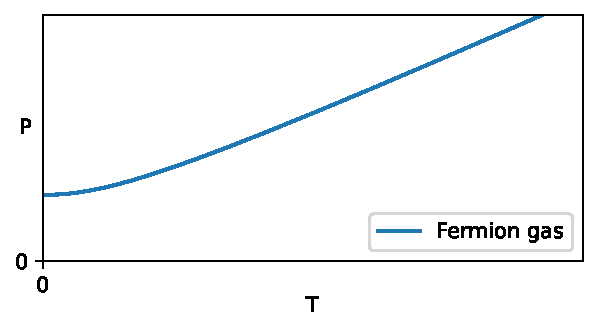
\includegraphics[width=0.725\textwidth]{figs/unit08_pressure.pdf}\end{center}
% ------------------------------------------------------------------



% ------------------------------------------------------------------
\subsection{Type-Ia supernovas}
The positive pressure that remains for a fermion gas even at zero temperature, \eq{eq:degen_pressure}, is known as the \textit{degeneracy pressure}.
(This use of the word `degenerate' is completely unrelated to its other use describing multiple energy levels with the same value of the energy.)
The degeneracy pressure plays a key role in a famous cosmic phenomenon---a certain class of supernova explosions of stars.

As a opening remark to this topic, note that the temperature doesn't need to be exactly zero in order for the degeneracy pressure to be significant.
The temperature just needs to be small compared to the Fermi energy, $T \ll E_F$.
From \eq{eq:Fermi_energy} we can see that $E_F \propto \rho_{\text{f}}^{2 / 3}$ increases for larger densities $\rho_{\text{f}} = \vev{N}_{\text{f}} / V$.
Not surprisingly, the densities of stars can be very large indeed, due to the enormous amount of matter that is being squeezed together by gravitational attraction.
Everyday matter has densities around $10^{28}$--$10^{29}$ atoms per cubic metre (roughly corresponding to Avogadro's number per cubic centimetre), which results in Fermi energies $E_F \sim 10^4$~K. % 2--10 eV with eV~10^4 K being the Boltzmann constant
Fermi energies for particularly dense stars known as \textit{white dwarfs} are a hundred thousand times larger, $E_F \sim 10^9$~K, corresponding to densities of roughly one tonne per cubic centimetre.
This is around a million times more dense than our sun---while white dwarf stars have a mass similar to our sun's $M_{\odot}$, their radius is a hundred times smaller, comparable to the radius of the earth.

White dwarf stars are so dense because they have exhausted the hydrogen and helium `fuel' for the nuclear fusion that generates heat and light---and therefore radiation pressure---in stars such as our sun.
For actively `burning' stars, this radiation pressure counteracts the gravitational attraction of the star's enormous mass.
Without nuclear fusion, white dwarfs end up gravitationally compressed into much denser and more compact objects.
The degeneracy pressure, \eq{eq:degen_pressure}, coming from the (fermionic) electrons in the white dwarf is what stabilizes these stars and prevents them from collapsing further into even denser objects such as black holes.

It is remarkable that even under these extreme conditions the electrons in white dwarf stars are well described by the non-interacting ideal fermion gas we have analyzed above.
In particular, it is crucial that white dwarfs' Fermi energies are so large, $E_F \sim 10^9$~K.
Even though white dwarfs have burned all their nuclear fuel, their interiors remain quite hot by everyday standards, roughly ten million kelvin ($T \sim 10^7$~K). % 0.3 MeV ~ 10^5 eV with eV~10^4 K being the Boltzmann constant
It is only due to their large densities and Fermi energies that $T \ll E_F$ and white dwarfs can be treated as zero-temperature objects to a good approximation.

So far we've seen no sign of supernovas.
In isolation, white dwarfs will happily cool for trillions of years, supported by their degeneracy pressure, until they reach thermal equilibrium with the $T_{\text{CMB}} \approx 2.725$~K cosmic microwave background radiation we considered last week. % TODO: CMB temperature will also keep decreasing as universe continues expanding...
Things become more interesting for a white dwarf that forms a binary system with a companion star.
If this companion star that is still burning hydrogen or helium through nuclear fusion, it will emit matter that is then captured by the white dwarf, slowly increasing the white dwarf's mass.
Such a binary system is pictured below, in an artist's illustration provided by the \href{https://www.esa.int/ESA_Multimedia/Images/2014/09/Artist_s_impression_of_Type_Ia_supernova}{European Space Agency}.

\begin{center}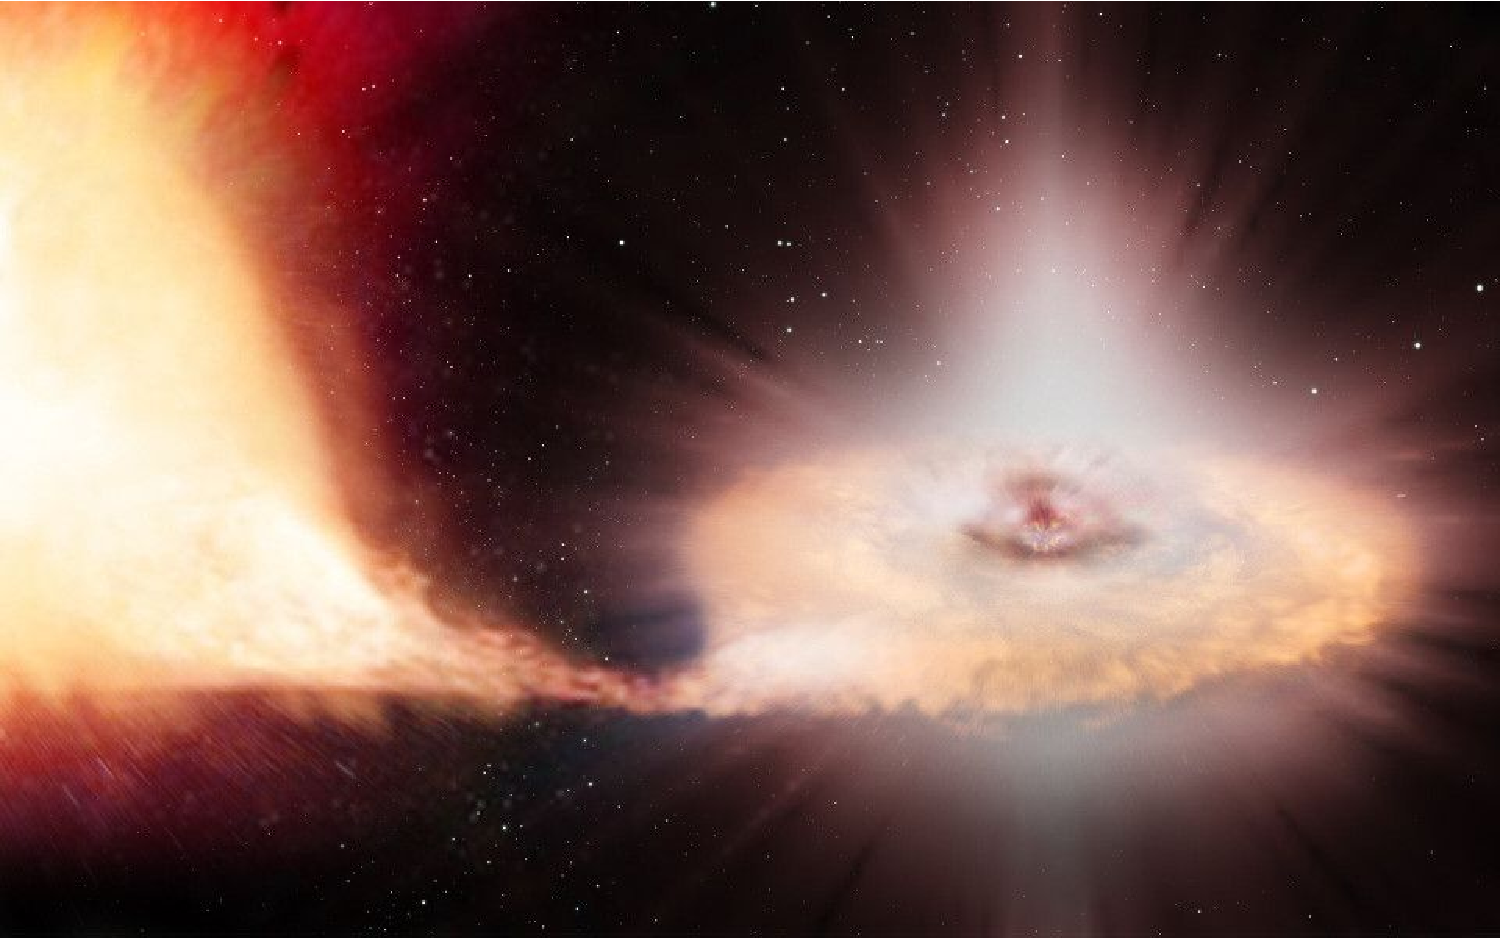
\includegraphics[width=0.8\textwidth]{figs/unit08_nova.pdf}\end{center}

As the white dwarf accumulates the matter emitted by its companion, its mass and its density will steadily increase.
As the mass of the white dwarf approaches a value about 40\% larger than the mass of our sun (known as the Chandrasekhar limit, named after \href{https://en.wikipedia.org/wiki/Subrahmanyan_Chandrasekhar}{Subrahmanyan Chandrasekhar}), its density becomes large enough for new types of nuclear fusion reactions to occur.
Instead of hydrogen or helium, which the white dwarf has already burned, these new fusion reactions involve carbon and oxygen, which the white dwarf has in plenty.
In the space of just a few seconds, these fusion reactions run away, increase the temperature of the white dwarf to billions of kelvin, and blast it apart in a supernova explosion about five billion times brighter than the sun.

For obscure historical reasons, these particular stellar explosions are known as \textit{type-Ia} (``one-A'') \textit{supernovas}.
They rely on the degeneracy pressure (\eq{eq:degen_pressure}) of a low-temperature gas of non-interacting fermions, which allows a specific amount of mass to build up before the explosion is triggered.
The specificity of the process results in a great deal of regularity among type-Ia supernovas, which is very useful to astronomers.
In particular, these type Ia supernovas play a key role in demonstrating that the expansion of the universe is accelerating (a phenomenon popularly called `dark energy'), which was awarded the 2011 Nobel Prize in Physics.
% ------------------------------------------------------------------



% ------------------------------------------------------------------
\subsection{Relativistic ideal fermion gas}
While our main focus this week is on non-relativistic gases with $E \propto p^2$, gases of relativistic fermions also appear in nature.
In fact, by changing units we can see that the white dwarf Fermi energy discussed above, $E_F \sim 10^9~\text{K} \sim 0.3$~MeV is comparable to the $0.511$~MeV rest-energy of electrons, suggesting that relativistic effects may be non-negligible in white dwarfs.
Such relativistic effects were indeed taken into account by Chandrasekhar and others investigating these compact stars in the twentieth century.
While the full calculations required to analyze massive relativistic particles are beyond the scope of this module, we can benefit from last week's consideration of gases of massless photons to briefly consider similar gases of massless fermions.
\textit{Neutrinos} (denoted `$\nu$') are physical examples of particles whose masses are so small that they can be very well approximated as massless fermions.\footnote{Neutrinos' masses are so small that it was extremely difficult to determine that they are not exactly massless.  The 2015 Nobel Prize in Physics was awarded for this discovery.}

In the same way as photons, such massless fermions travel at the speed of light, $c$, and have energies $E = cp$ that depend on their angular frequencies,
\begin{equation}
  E_{\nu} = \hbar \om.
\end{equation}
In a volume $V = L^3$, these energies are quantized as usual,
\begin{equation*}
  \om = \frac{2\pi c}{\la} = c \frac{\pi}{L} k,
\end{equation*}
where $k^2 = k_x^2 + k_y^2 + k_z^2$ and $k_{x, y, z} > 0$ are positive integers.
Just as for the massive fermions considered in \secref{sec:fermi_nonrel}, for each distinct set of integers $\vec k = (k_x, k_y, k_z)$, typical massless fermions such as neutrinos have two degenerate energy levels with the same energy.

The detailed analysis of a gas of massless fermions is nearly the same as the work we did last week for photon gases.
In particular, massless fermions are also well described by a vanishing chemical potential, $\mu \approx 0$.
Again approximating sums over discrete integer $k_{x, y, z}$ by integrals over continuous real $\khat_{x, y, z}$, and changing variables to integrate over the angular frequency, we end up with the grand-canonical potential
\begin{align}
  \Phi_{\nu} = -\frac{VT}{c^3 \pi^2} \int_0^{\infty} d\om \; \om^2 \log\left[1 + e^{-\be \hbar \om}\right]. \label{eq:neutrino_grand}
\end{align}
The only change in $\Phi_{\nu}$ compared to \eq{eq:photon_grand} for photons are a couple of negative signs, precisely as we would expect from comparing the Bose--Einstein and Fermi--Dirac grand-canonical potentials in \secref{sec:quantum_classical}.

Carrying out the derivatives to obtain the average particle number density and the average internal energy density produces
\begin{align}
  \frac{\vev{E}_{\nu}}{V} & = \frac{1}{c^3 \pi^2} \int_0^{\infty} \frac{\hbar \om^3}{e^{\be \hbar \om} + 1} d\om &
  \frac{\vev{N}_{\nu}}{V} & = \frac{1}{c^3 \pi^2} \int_0^{\infty} \frac{\om^2}{e^{\be \hbar \om} + 1} d\om,
\end{align}
now differing only by negative signs in their denominators compared to the photon gas results we obtained last week.
The condition of constant entropy is still $V T^3 = \mbox{constant}$, and the resulting pressure leads to an equation of state in the usual form,
\begin{equation*}
  P_{\nu} V \propto \vev{N}_{\nu} T,
\end{equation*}
with the constant of proportionality another $\cO(1)$ number involving the Riemann zeta function.
% ------------------------------------------------------------------
